\documentclass[12pt,a4paper]{report}
\usepackage[portuguese,brazil]{babel}
\usepackage[utf8]{inputenc}
%\usepackage[T1]{fontenc}
\usepackage{graphicx}
%\usepackage{indentfirst}
\usepackage{fancyhdr}
\usepackage{algorithm-br}
\usepackage{algorithmic-br}


% hiperlinks
\usepackage[backref,pdfpagemode=UseOutlines,colorlinks=true,
a4paper,breaklinks=true,hyperindex,linkcolor=red,
anchorcolor=black,citecolor=green,filecolor=magenta,
menucolor=red,pagecolor=red,urlcolor=blue,bookmarks=true,
bookmarksopen=true,pdfpagelayout=SinglePage,
pdfpagetransition=Dissolve]{hyperref}


% format
\setlength{\parskip}{.2cm}
\setlength{\textwidth}{16cm}
\setlength{\textheight}{23 cm}
\setlength{\topmargin}{0cm} 
\setlength{\oddsidemargin}{0.5cm}
\setlength{\evensidemargin}{0.5cm} 


\begin{document}
\sloppy

\pagestyle{empty}
\vspace*{\stretch{1}}

\begin{center}
\noindent \rule{\linewidth}{.1cm}

\vspace*{1cm}

{\LARGE \textsf{Um Algoritmo Genético para o Problema da Mochila Compartimentada}}

\vspace*{1cm}

{\Large \textsf{Pedro Henrique Neves da Silva}}

\vspace*{1cm}

\noindent \rule{\linewidth}{.1cm}

\vspace*{1cm}

{\large

\textbf{Departamento de Computação e Estatística} \\
\textbf{Universidade Federal de Mato Grosso do Sul}

}

\vspace*{1cm}

\begin{figure}[htb]
\begin{center}
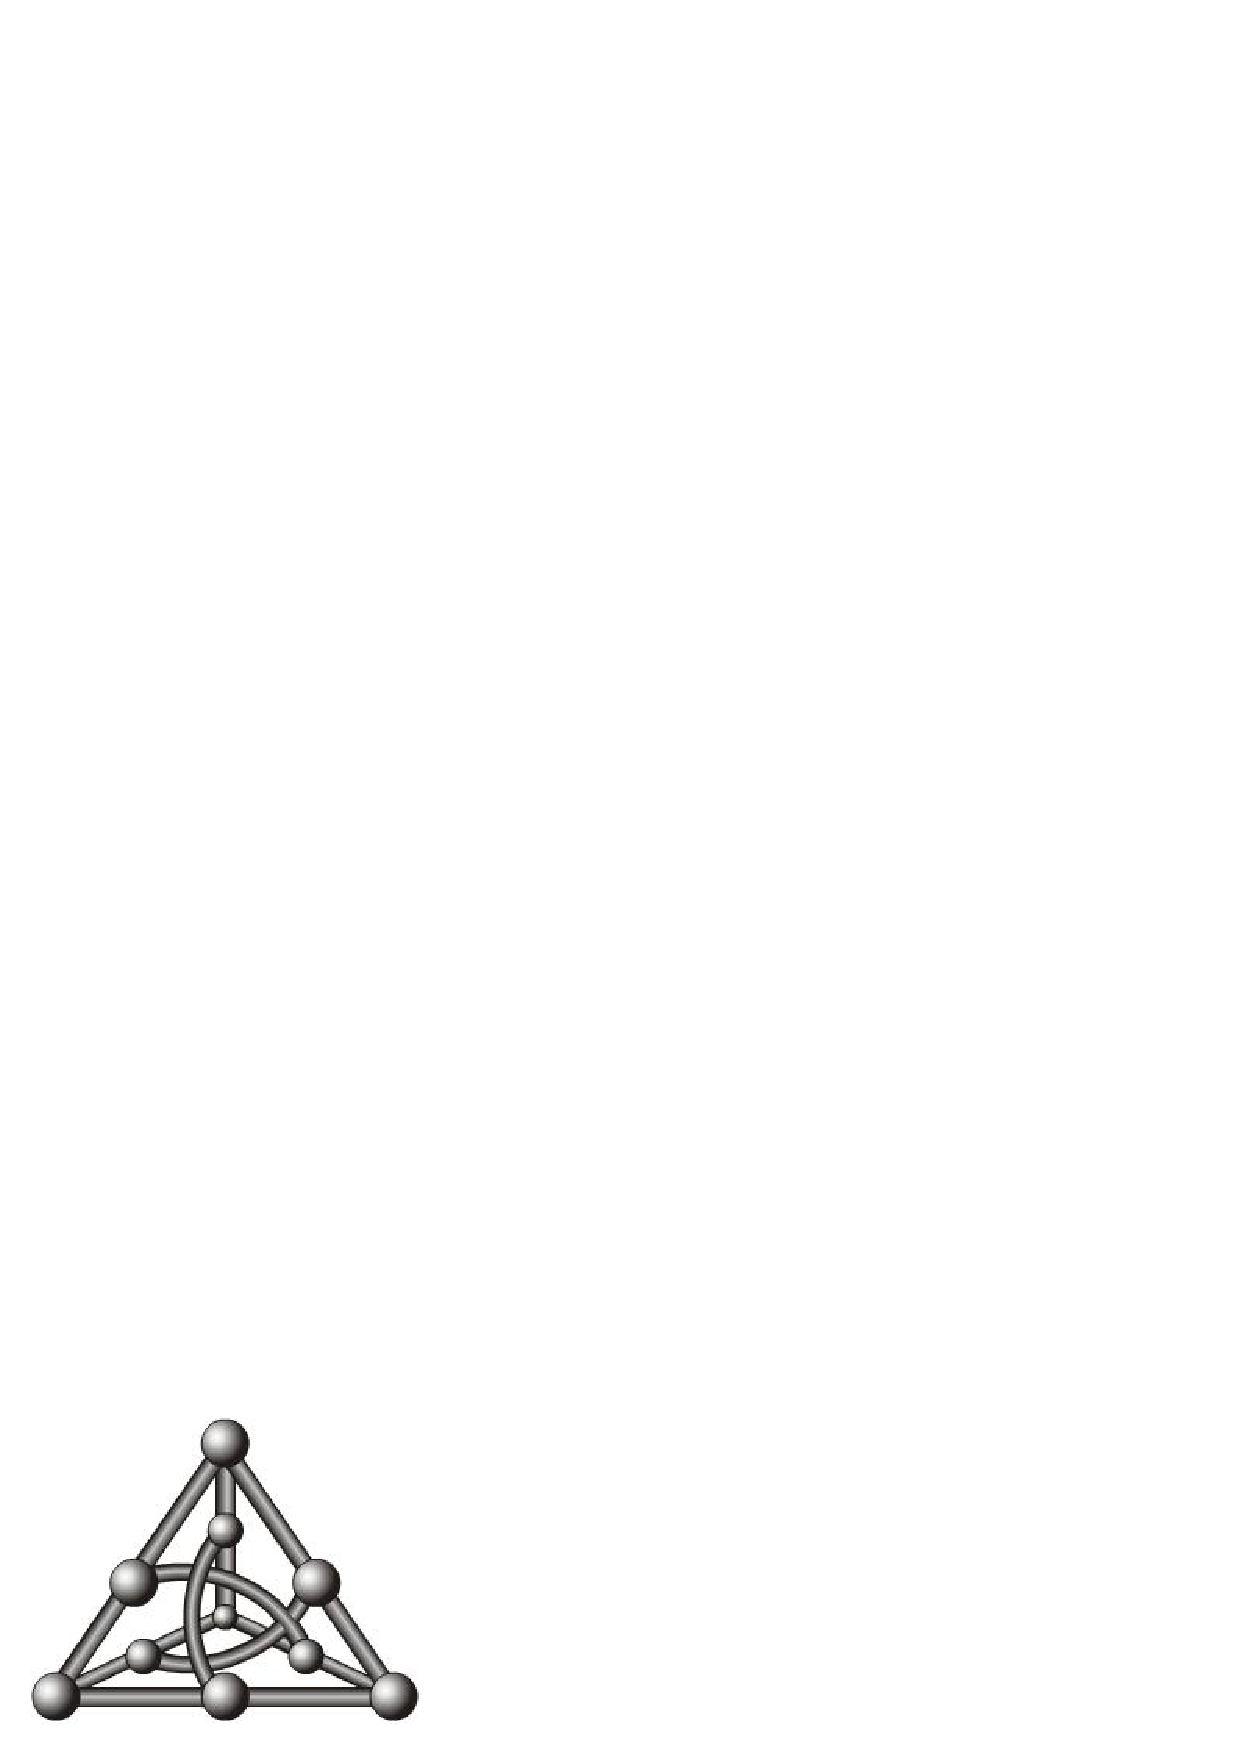
\includegraphics[width=4cm]{images/grafo.pdf}
\end{center}
\end{figure}
\vspace{2 cm}

\textbf{Orientadora: Prof. Ms. Liana Duenha}

\vspace*{\stretch{2}}

Campo Grande, Agosto de 2009

\end{center}

\newpage




\pagenumbering{roman}
\setcounter{page}{1}

\newpage
\tableofcontents
\newpage

\pagestyle{fancy}
\pagenumbering{arabic}
\renewcommand{\chaptermark}[1]{\markboth{#1}{}}
\renewcommand{\sectionmark}[1]{\markright{\thesection\ #1}}


\setcounter{page}{1}


\pagestyle{plain}

\begin{abstract}
O Problema da Mochila é um dos problemas de otimização combinatória mais estudados da classe NP-difícil. Este trabalho aborda uma variação do problema original, conhecida como Problema da Mochila Compartimentada, onde os itens são divididos em classes e a mochila pode ser dividida em compartimentos, de tal forma que cada compartimento armazene itens de uma mesma classe. O problema consiste de encontar a distribuição dos itens em compartimentos que maximize o valor de utilidade da mochila, obedecendo restrições quanto à capacidade máxima da mochila e de cada compartimento. O  principal resultado deste trabalho refere-se a apresentação de um algoritmo genético para o Problema da Mochila 0-1 e para o Problema da Mochila Compartimentada, incluindo divulgação dos resultados de experimentação e comparação destes algoritmos com outros que utilizam estratégicas convencionais para resolução dos mesmos problemas.
%Existem muitas abordagens para obter uma solução aproximada em tempo polinomial. Aqui nós consideraremos o clássico problema da mochila 0/1 e uma %variação desse problema, o problema da mochila compartimentada. No segundo problema, temos que determinar as capacidades adequadas de vários %compartimentos que podem vir a ser alocados em uma mochila e como esses compartimentos devem ser carregados.

\end{abstract}

\chapter*{Introdução} \label{sec:introducao}
O Problema da Mochila desperta muito interesse devido a sua vasta gama de aplicações e também pelo fato de que ele surge como subproblema de inúmeros outros problemas. Devido a sua importância, ele é amplamente estudado, possuindo diversas variantes agrupadas no que podem ser chamadas de Classes de Problemas da Mochila.

Ele se caracteriza, basicamente, pela escolha de um subconjunto de itens que irá otimizar um objetivo. Para tanto, cada item deve possuir um ``peso'' e um ``benefício'' e a mochila deve possuir uma capacidade máxima.  Deseja-se, então, escolher um subconjunto de itens que maximize o benefício da mochila, sem que a soma dos pesos dos itens selecionados ultrapasse a capacidade da mochila.

Neste projeto, além do clássico Problema da Mochila 0-1, mostramos uma variação do mesmo, chamado Problema da Mochila Compartimentada, onde a mochila pode ser dividida em compartimentos que, por sua vez, agrupam itens de uma mesma classe ou tipo. Esse problema foi proposto em 1996 e, embora não tenha uma solução polinomial, é de interesse que existam heurísticas ou algoritmos aproximativos para resolvê-lo rapidamente já que o problema possui várias aplicações práticas, incluindo a aplicação na indústria metalúrgica, que motivou sua proposta inicial.

Este trabalho está dividido da seguinte forma: no Capítulo~\ref{sec:mochila}, definimos e explicamos algumas das classes de Problemas da Mochila, bem como algumas técnicas tradicionais de projeto de algoritmos para resolução de alguns dos problemas apresentados. Este capítulo também apresenta os principais conceitos relacionados aos Algoritmos Genéticos. No Capítulo~\ref{sec:compartimentada}, definimos o Problema da Mochila Compartimentada e descrevemos uma forma de resolução do problema utilizando a Heurística da Decomposição. No mesmo capítulo, apresentamos uma simplificação do problema, e um possível algoritmo genético resolvê-lo.

No Capítulo~\ref{sec:resultados}, descrevemos todas as implementações e experimentações realizadas. Apresentamos três métodos de resolução do Problema da Mochila 0-1, um método utilizando força bruta para o Problema da Mochila Compartimentada e dois algoritmos genéticos, um para a resolução do Problema da Mochila 0-1 e o outro para o Problema da Mochila Compartimentada. Este capítulo inclui comparações relacionadas ao tempo de execução dos principais métodos e a comparação entre as soluções retornadas pelos algoritmos genéticos e pelos algoritmos exatos também implementados. Por fim, no capítulo~\ref{sec:conclusao}, apresentamos as considerações finais e o resumo dos principais resultados obtidos. 


\pagestyle{plain}

\chapter{Problemas da Mochila} \label{sec:mochila}

Existem diversas versões de Problemas da Mochila, todos elas caracterizadas por selecionar, dentre um conjunto de objetos ou itens disponíveis, um subconjunto que irá otimizar uma função objetivo, satisfazendo determinadas restrições. Para tanto, cada item deve possuir um {\it ``peso''} e um {\it ``benefício''}. Por peso entende-se uma penalidade a ser paga pela inclusão do item. É comum encontrar o termo ``penalidade'' ou ``custo'' para expressar o peso de um item. Por ``benefício'' entende-se a utilidade ou lucro obtido pela escolha do item e esse valor contribuirá no objetivo do problema. 

A principal restrição imposta nos problemas da mochila relaciona-se à sua capacidade. De fato, a soma do peso dos itens selecionados deve respeitar a capacidade da mochila. Geralmente, expressamos capacidade da mochila e custo dos itens utilizando a mesma unidade de medida. Várias outras restrições ou condições podem ser impostas no problema e cada nova restrição agrega um custo computacional para encontrar sua solução. O Problema da Mochila, em sua versão mais simples, é integrante da classe NP-difícil \cite{GJ79}. Consequentemente, várias outras versões do Problema da mochila, várias delas apresentadas nesse texto, pertencem também à mesma classe de problemas.

Neste capítulo são apresentadas várias classes de Problemas da Mochila, incluindo descrição e modelo matemático, com o objetivo de ilustrar a diversidade de problemas relacionados. Essa fundamentação será útil para que nos próximos capítulos seja estudada a versão de Problemas da Mochila de maior interesse neste trabalho, conhecida como Problema da Mochila Compartimentada. Ainda no capítulo veremos os principais métodos e técnicas de resulução computacional dos problemas da mochila, incluindo alguns algoritmos para exemplificação. 

\section{Classes de Problemas da Mochila}

Todas as mochilas que serão apresentados nessa seção utilizam um conjunto de itens $S$ com $n$ itens, cada item $i$ ($1 \leq i \leq n$) deve estar associado a um valor de benefício $b_i$ e um peso $l_i$. A capacidade da mochila é representada por $L$. 


\subsection{Problema da Mochila 0-1} \label{m01}

Para cada item $i \in S$ é associada a variável $x_i$ que pode assumir um dos dois valores: 0 ou 1. $x_i$ será 0 quando o item $i$ não for escolhido para compor a mochila, e será 1 quando o item fizer parte da solução. Por esse motivo, essa versão também é conhecida como mochila binária. Segue abaixo o modelo matemático:

\hspace*{3.0cm} Maximize:
\begin{equation}
 \sum_{i=1}^n b_i x_i 
\end{equation} 

\hspace*{3.0cm} Sujeito a:
\begin{equation}
 \sum_{i=1}^n l_i x_i  \leq L
\end{equation} 

\begin{equation}
 x_i=0 \textrm{ ou } 1, i=1,...,n 
\end{equation} 

Algumas informações com relação ao conjunto de itens podem ser observadas. Por exemplo, nenhum item do conjunto $S$ deve possuir peso maior do que a capacidade máxima da mochila, pois, caso contrário, esse item não faria parte de nenhuma solução do problema. Outro ponto importante sobre o conjunto de itens é que a soma dos pesos dos itens de $S$ não pode ser menor que $L$, já que desta forma a solução ótima seria a soma dos benefícios de todos os itens. 

\subsection{Versão Fracionária do Problema da Mochila} \label{frac}

Se não houver a restrição de {\it aceitar} ou {\it recusar} um item de $S$ para fazer parte da solução, e tivermos a possibilidade  de escolher uma porção do item para fazer parte da solução, teremos a versão fracionária do Problema da Mochila. Nessa versão, permite-se escolher pedaços arbitrários de alguns elementos. Deseja-se, então, encontrar a porção $x_i$ do item $i$ que fará parte da solução, tal que

\begin{equation}
 0 \leq x_i \leq l_i \textrm{ para cada } i\in S \textrm{ e } \sum_{i=1}^n x_i \leq L 
\end{equation}

O benefício total do conjunto de itens é determinado pela função objetivo

\begin{equation}
 \sum_{i \in S} b_i(x_i/l_i)
\end{equation}

Essa versão do problema possui uma solução bastante simples utilizando a abordagem gulosa, ordenando o conjunto de itens pelo valor $b_i/l_i$ e fazendo com que os itens com maior valor $b_i/l_i$ sejam escolhidos primeiro até que não seja mais possível incluir um item por completo. Seja $j$ $(0 \leq j \leq n)$ o último item avaliado e inserido por completo na solução e seja $l$ o somatório dos pesos dos itens já inseridos até o momento.  A porção do item $j+1$, se tal item existir, que fará parte da solução será $x_{j+1} = L-l$. 

Por ter uma solução polinomial bastante simples, esta versão do problema não se enquadra na classe de problemas que estamos estudando neste trabalho. Porém, na seção ~\ref{bb}, utiliza-se a abordagem gulosa descrita acima em um método heurístico para cálculo de um limitante superior para o valor da solução ótima, que será utilizado em um algoritmo {\it branch and bound} para solucionar do Problema da Mochila 0-1. 



\subsection{Problema da Mochila Restrita}

Na classe de mochilas restritas, as variáveis deixam de ser binárias e passam a indicar o número de repetições do respectivo item na mochila. Além do mais, cada variável têm associada a ela um limitante inferior e um superior. No modelo matemático desta classe, $d_i$ e $t_i$ representam o limitante superior e o limitante inferior para o item $i$, respectivamente. 

\hspace*{3.0cm} Maximize:
\begin{equation}
 \sum_{i=1}^n b_i x_i 
\end{equation} 

\hspace*{3.0cm} Sujeito a:
\begin{equation}
 \sum_{i=1}^n l_i x_i  \leq L
\end{equation} 

\begin{equation}
 t_i \leq x_i \leq d_i \textrm{ e inteiro }, i=1,...,n 
\end{equation} 

Por questões de simplicidade, pode ser necessário definir o limitante inferior como zero. Dado um problema definido como no modelo anterior, basta somar $(t_i*t_i)$ na função objetivo, subtrair $(l_i * t_i)$ de $L$ e $t_i$ de $d_i$, e finalmente, atualizarmos $t_i$ para zero. Com essa simples transformação sempre teremos zero como limitante inferior. 

Outra observação importante é que toda mochila restrita pode ser transformada em uma mochila 0-1. Um método para realizar essa transformação é ilustrado por~\cite{MT90}.

\subsection{Problema da Soma de Subconjuntos}

Esse tipo de mochila se aproxima muito da classe de mochilas com variáveis binárias. A diferença se restringe à função objetivo onde o benefício é substituído pelo peso do item. Esta nova abortagem é útil quando é necessário selecionar um subconjunto de itens, cuja soma de seus pesos se aproxime ao máximo, mas não exceda, a capacidade da mochila.  Segue o modelo matemático equivalente:

\hspace*{3.0cm} Maximize:
\begin{equation}
 \sum_{i=1}^n l_i x_i 
\end{equation} 

\hspace*{3.0cm} Sujeito a:
\begin{equation}
 \sum_{i=1}^n l_i x_i  \leq L
\end{equation} 

\begin{equation}
 x_i=0 \textrm{ ou } 1, i=1,...,n 
\end{equation} 

Esse problema pode surgir, por exemplo, nessas circunstâncias: considere um servidor de internet e um conjunto de pedidos de download. Para cada pedido de download, podemos determinar o tamanho do arquivo solicitado e, por isso, podemos sintetizar cada pedido como um valor inteiro (representando o tamanho do arquivo solicitado). Dado esse conjunto de inteiros, pode ser interessante determinar um subconjunto deles que, quando somados, tenham a largura de banda de nosso servidor durante uma fração de tempo. Esse problema é uma instância do problema da soma de subconjuntos. 

Infelizmente, fica mais difícil resolver esse problema à medida que a largura de banda e a capacidade de atender pedidos aumentam. Esse é um problema da classe NP-completo e a demonstração de que, de fato, pertence a esta classe de problemas encontra-se em~\cite{MTG02}.

\subsection{Problema de Múltiplas Mochilas 0-1}

No Problema de Múltiplas Mochilas considera-se $n$ conjuntos de itens, disjuntos entre si, e um conjunto com $m$ mochilas, cada uma com capacidade $L_j$ $(1 \leq j \leq m)$. O problema consiste em atribuir itens que fornecerão o maior benefício possível, considerando que os itens de um determinado conjunto podem ser atribuídos a, no máximo, uma única mochila. Nesse caso, a variável de decisão $x_{ij}=1$, se o item $i$ foi adicionado à mochila $j$. Caso contrário, $x_{ij}=0$. 

\hspace*{3.0cm} Maximize:
\begin{equation}
 \sum_{j=1}^m \sum_{i=1}^n b_i x_{ij} 
\end{equation} 

\hspace*{3.0cm} Sujeito a:
\begin{equation}
 \sum_{i=1}^n l_i x_{ij} \leq L_j, j=1,...,m
\end{equation} 

\begin{equation}
 \sum_{j=1}^m x_{ij} \leq 1, i=1,...,n
\end{equation} 

\begin{equation}
 x_{ij}=0 \textrm{ ou } 1, i=1,...,n , j=1,...,m 
\end{equation} 

Quando $n=1$, o Problema de Múltiplas Mochilas 0-1 se reduz a um Problema da Mochila 0-1 original.


\section{Estratégias para Resolução de Mochilas} \label{cap2_tec_estr}

Embora o Problema da Mochila 0-1 e suas variações sejam pertencentes à classe NP-difícil, muitos deles surgem em aplicações práticas na vida real ou como sub-problemas de outros problemas mais complexos e por isso justifica-se a tentativa de encontrar soluções exatas ou aproximadas, mesmo que isso custe muito tempo. Nesta seção abordaremos as principais técnicas de projeto de algoritmos utilizadas para resolver de maneira exata ou aproximada alguns Problemas da Mochila. 

\subsection{Branch and Bound} \label{bb}

Esta técnica apresenta-se como um método geral para encontrar soluções ótimas para problemas de otimização combinatória. Esse método tem como entrada uma instância para um problema difícil de otimização e como saída uma solução ótima, se existir. A estratégia usando força-bruta é buscar sistematicamente em um grande (possivelmente exponencial) conjunto de possibilidades, computar o valor associado a cada possível configuração e devolver a melhor das configurações encontradas de acordo com uma função objetivo de maximização ou minimização. A técnica {\it branch-and-bound} utiliza o mesmo método, porém inclui um mecanismo para diminuir o conjunto de possibilidades, descartando a verificação daquelas configurações que não tenham chance de serem soluções ótimas, melhorando o tempo de resposta do algoritmo. Para descartar configurações não promissoras, calcula-se um {\it limitante} que é o valor máximo (para problemas de maximização) ou mínimo (para problemas de minimização) que uma solução pode atingir a partir da configuração em questão. Se esse valor limitante não for satisfatório, essa configuração  (e consequentemente, todas que seriam atingidas no espaço de busca a partir dela) será descartada. A dificuldade inerente a esta técnica está no fato de que quanto melhor for definido o limitante, melhor o tempo de resposta do algoritmo.

Para explicar como aplicar a técnica {\it branch and bound},  considera-se, nesse contexo, o Problema da Mochla 0-1, descrita na subseção ~\ref{m01}. Um limitante será definido utilizando uma abordagem gulosa, similar à técnica utilizada para resolver a versão fracionária do Problema da Mochila, descrita na seção ~\ref{frac}. Assume-se que os itens do conjunto $S$ sejam colocados em ordem não-decrescente, pelo valor de $b_i/l_i$. Eles serão processados nesta ordem, pois assim estaremos considerando os itens na ordem de benefício/custo decrescente, começando com o elemento de maior benefício/custo. Nossa configuração é definida pelo subconjunto $S_i$ dos primeiros $i$ itens de $S$ baseados nesta ordem. Assim, os índices dos itens de $S_i$ estão entre 0 e $i-1$, e podemos definir o conjunto $S_0$ como uma configuração vazia. 

Iniciamos colocando a configuração $S_0$ em uma fila de prioridades $P$ e, a cada iteração do algoritmo, escolhemos a configuração mais promissora $c$ em $P$. Se $i$ é o índice do último item considerado em $c$, então expandimos $c$ em duas novas configurações: uma que inclui o item $i+1$ e uma que não o inclui. Note que cada configuração satisfatória à restrição de tamanho é uma configuração válida para o problema em questão. Assim, se qualquer uma das duas configurações for válida e melhor do que a melhor solução encontrada até o momento, atualizamos nossa melhor opção corrente e continuamos o processo. 

Para escolher configurações que sejam mais promissoras, precisamos ter uma forma de avaliá-las por seu valor potencial. Para tanto, utilizaremos um limite superior para o seu valor potencial: dada uma configuração $c$ que considera os itens de índice $0$ a $i$, calculamos um limite superior para $c$ iniciando com o valor total $l_c$ de $c$ e verificando quanto valor a mais podemos colocar em $c$ se aumentarmos $c$ com uma solução para o problema fracionário da mochila que seja retirada dos itens restantes em $S$. Seja $k$ o maior índice tal que $\sum_{j=i+1}^{k} s_j \leq L-s_c$, onde $s_c$ é o somatório dos pesos de todos os itens que compõem na configuração $c$. Os itens de $i+1$ a $k$ são os melhores itens que ainda cabem na mochila. Para calcular o limite superior para $c$, consideramos a adição de todos esses elementos a $c$ mais tudo o que for possível do item $k+1$ (se existir). Nosso limite superior $upper(c)$ para $c$ será então definido como segue:


\begin{equation}
 upper(c)= l_c+ \sum_{j=i+1}^{k} l_j + (L-s_c-\sum_{j=i+1}^{k} s_j) (l_{k+1})/(s_{k+1})
\end{equation} 

Se $k=n-1$, então assumimor que $(l_{k+1})/(s_{k+1}) = 0$.

No capítulo seguinte mostraremos os resultados obtidos por meio da implementação da técnica descrita para solucionar o Problema da Mochila 0-1 utilizando {\it branch-and-bound} e avaliaremos seu desempenho com relação aos outros métodos implementados.



\subsection{Programação Dinâmica} \label{progdin}


A proposta mais simples e promissora para resolver o Problema da Mochila 0-1 é utilizar programação dinâmica. Inicialmente, os itens de $S$ serão numerados como 1,2,3,...,$n$ e para cada $k \in \{1,2,...,n\}$, defini-se $S_k$ como o subconjunto contendo itens $S$ rotulados de 1 até $k$.

Formulamos, então, cada subproblema como sendo o cálculo de $B[k,w]$, que é definido como o valor total máximo (benefício total) de um subconjunto
$S_k$ entre todos os subconjuntos que têm seus pesos totais até $w$. Teremos $B[0,w]$=0 para cada $w \leq W$ e derivaremos a seguinte
relação para o caso geral:


\[ B[k,w]= \left \{ \begin{tabular}  {lc}
                                     $B[k-1,w]$ & $:l_k > w$ \\
                                     $max\{ B[k-1,w], B[k-1,w-l_k]+b_k\}$ & $:l_k \leq w$ \\
                                  \end{tabular} \right. \]


Ou seja, $B[k,w]$ é o melhor subconjunto $S_k$ cujo peso total $w$ é ou o melhor subconjunto de $S_{k-1}$ que tem o peso total $w$ ou o melhor
subconjunto de $S_{k-1}$ que tem peso total $w-l_k$ mais o item $k$. Uma vez que o melhor subconjunto de $S_k$ com o peso total $w$ deva ou não conter o item $k$, uma dessas duas escolhas será a melhor.

\begin{algorithm}
\caption{Mochila\_Programção\_Dinâmica} %titulo do algoritmo
\label{alg2}
\begin{algorithmic}[1]
 
	\REQUIRE Conjunto $S$ de $n$ itens, tais que o item $i$ tem um benefício positivo $b_i$ e um peso inteiro positivo $l_i$, um inteiro positivo $L$ que corresponde ao peso total da mochila.
 
	\ENSURE Para $w=0,...,L$, o benefício máximo $B[w]$ de um subconjunto de $S$ com peso total $w$.

	\FOR {$w \leftarrow 0$ \ até \ $L$}
		\STATE $B[w] \leftarrow 0$
	\ENDFOR
	\FOR {$k \leftarrow 1$ \ até \ $n$}
		\FOR{$w \leftarrow L$ \ descrescendo \ até \ $l_k$}
			\IF{$B[w-l_k]+b_k > B[w]$}
				\STATE $B[w] \leftarrow B[w-l_k]+b_k$
			\ENDIF
		\ENDFOR
	\ENDFOR
\end{algorithmic}
\end{algorithm}

O tempo de execução do algoritmo é determinado pelos dois laços aninhados, onde o mais externo tem $n$ iterações e o mais interno tem no máximo $L$ iterações. Desta forma, poderemos determinar o valor ótimo localizando o maior entre todos os elementos do vetor $B$. Assim, podemos encontrar o subconjunto de $S$ de maior benefício com peso total de no máximo $L$ em tempo $O(nL)$. 

Considera-se que é um algoritmo de complexidade de tempo pseudo-polinomial, já que depende, além da quantidade de itens do conjunto $S$, da magnitude de um número fornecido na entrada. Porém, na prática, esse algoritmo comporta-se muito melhor do que o algoritmo de força bruta (exponencial). No capítulo seguinte mostramos os resultados referentes à implementação desse método e avaliaremos o seu desempenho com relação aos outros métodos também implementados.


\subsection{Algoritmos Genéticos} \label{algen}

Os algoritmos genéticos são uma família de modelos computacionais inspirados na evolução, indicados para encontrar soluções aproximadas para problemas de otimização difíceis, como o Problema do Caixeiro Viajante, Problemas de Satisfabilidade ou Problemas da Mochila, que envolvem um grande número de variáveis e, consequentemente, espaços de soluções de dimensões elevadas ~\cite{Wei09}. Nesta seção, mostraremos os conceitos relacionados a esta técnica a fim de fundamentar a proposta de um algoritmo genético para encontrar uma solução aproximada para o Problema da Mochila 0-1 e sua extensão para o Problema da Mochila Compartimentada.

Embora existam variações de acordo com a aplicação, algoritmos genéticos simples normalmente trabalham com descrições de entrada formadas por cadeias de bits de tamanho fixo.  Há três tipos de representação possíveis: binária, inteira ou real. A essa representação se dá o nome de {\it alfabeto} do algoritmo. De acordo com a classe de problema que se deseje resolver pode-se usar qualquer um dos três tipos. Neste trabalho, utilizaremos alfabeto binário. 

Uma implementação de um algoritmo genético começa com uma população aleatória de cromossomos. Essas estruturas são, então, avaliadas e associadas a uma probabilidade de reprodução de tal forma que as maiores probabilidades são associadas aos cromossomos que representam uma melhor solução para o problema de otimização do que àqueles que representam uma solução pior.

Os principais conceitos envolvidos na implementação de algoritmos genéticos que foram utilizados para elaboração de um algoritmo genético para solucionar Problemas da Mochila neste trabalho são:
\begin{itemize}
\item {\bf gene:} um ou mais símbolos do alfabeto (neste trabalho, um gene corresponde a um símbolo do alfabeto binário)
\item {\bf cromossomo:} conjunto de genes que corresponde a um indivíduo
\item {\bf população:} conjunto de cromossomos (ou indivíduos) que corresponde ao conjunto de pontos no espaço de busca 
\item {\bf geração:} iteração completa do algoritmo genético que gera uma nova população 
\item {\bf aptidão bruta:} saída gerada pela função objetivo para um indivíduo da população 
\item {\bf aptidão máxima:} melhor aptidão encontrada para indivíduos da população corrente 
\item {\bf aptidão média:} aptidão média da população corrente 
\end{itemize}

Deve ser observado que cada cromossomo, chamado de indivíduo no algoritmo, corresponde a um ponto no espaço de soluções do problema de otimização. O processo de solução adotado nos algoritmos genéticos consiste em gerar, através de regras específicas, um grande número de indivíduos (população), de forma a promover uma varredura tão extensa quanto necessária do espaço de soluções. 

\begin{figure}[htp]
	\centering
	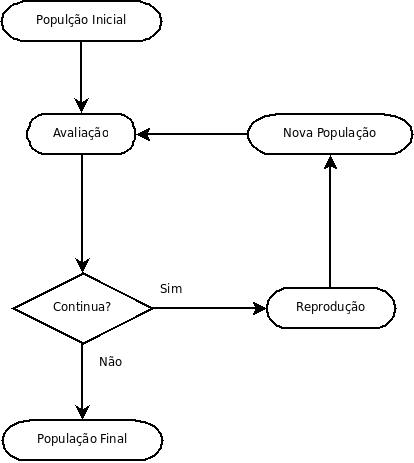
\includegraphics[scale=0.5]{images/fluxo.jpg}
	\caption{Fluxograma do algoritmo genético.}
	\label{fig:fluxo}
\end{figure}

Uma população de  indivíduos é gerada aleatoriamente. Cada um dos indivíduos da população representa uma possível solução para o problema, ou seja, um ponto no espaço de soluções. 
Cada iteração do algoritmo genético corresponde à aplicação de um conjunto de quatro operações básicas: cálculo de aptidão, seleção, cruzamento e mutação. Ao fim destas operações cria-se uma nova população, chamada de geração que, espera-se, representa uma melhor aproximação da solução do problema de otimização que a população anterior. A população inicial é gerada atribuindo-se aleatoriamente valores aos genes de cada cromossomo. A aptidão bruta de um indivíduo da população é medida por uma função, também chamada de função objetivo do problema de otimização.
Como critérios de parada do algoritmo em geral são usados a aptidão do melhor indivíduo em um conjunto com a limitação do número de gerações. 

\subsubsection{Cálculo de Aptidão}

Geralmente a aptidão do indivíduo é determinada por meio do cálculo da função objetivo, que depende das especificações de projeto. Os indivíduos são, então, ordenados conforme seus valores de aptidão bruta. A aptidão média é um valor associado á população e poderá ser calculado nessa etapa do algoritmo. Esse valor pode ser útil para avaliar e comparar populações, se necessário.

\subsubsection{Fase de Seleção}

Nesta fase os indivíduos mais aptos da geração atual são selecionados. Esses indivíduos são utilizados para gerar uma nova população por cruzamento. Cada indivíduo tem uma probabilidade de ser selecionado proporcional à sua aptidão. 

\subsubsection{Fase de Cruzamento ou ``CROSS-OVER''} 

Os indivíduos selecionados na etapa anterior são cruzados da seguinte forma: a lista de indivíduos selecionados é embaralhada aleatoriamente criando-se, desta forma, uma segunda lista, chamada lista de parceiros. Cada indivíduo selecionado é então cruzado com o indivíduo que ocupa a mesma posição na lista de parceiros. Os cromossomos de cada par de indivíduos a serem cruzados são particionados em um ponto, chamado ponto de corte, sorteado aleatoriamente. Um novo cromossomo é gerado permutando-se a metade inicial de um cromossomo com a metade final do outro. 

\subsubsection{Fase de Mutação}

A operação de mutação é utilizada para garantir uma maior varredura do espaço de estados. A  mutação é efetuada alterando-se o valor de um gene de um indivíduo sorteado aleatoriamente com uma determinada probabilidade, denominada probabilidade de mutação, ou seja, vários indivíduos da nova população podem ter um de seus genes alterado aleatoriamente. 

\subsubsection{Outros parâmetros}

Além da forma como o cromossomo é codificado, existem vários parâmetros do algoritmo genético que podem ser escolhidos para melhorar o seu desempenho, adaptando-o às características  particulares de determinadas classes de problemas.  Entre eles os mais importantes são: o tamanho da população, o número de gerações, a probabilidade de ``cross-over''  e a probabilidade de mutação. 
A influência de cada parâmetro no desempenho do algoritmo depende da classe de problemas que se está tratando. Assim, a determinação de um conjunto de valores otimizado para estes parâmetros dependerá da realização de um grande número de experimentos e testes. Na maioria da literatura os valores encontrados estão na faixa de 60 a 75\% para a probabilidade de cross-over e entre 0,1 e 5\% para a probabilidade de mutação. O tamanho da população e o número de gerações dependem da complexidade do problema de otimização e devem ser determinados experimentalmente. No entanto, deve ser observado que o tamanho da população e o número de gerações definem diretamente o tamanho do espaço de busca a ser coberto. Existem estudos que utilizam um algoritmo genético  como método de otimização para a escolha dos parâmetros de outro algoritmo genético, devido à importância da escolha correta destes parâmetros.


\pagestyle{plain}

\chapter{Problema da Mochila Compartimentada} \label{sec:compartimentada}

O Problema da Mochila Compartimentada é uma variação do Problema da Mochila. Este problema consiste em determinar as capacidades adequadas de vários compartimentos que podem vir a ser alocados em uma mochila e como esses devem ser carregados, respeitando as capacidades dos compartimentos e da mochila.

\section{Definição do Problema}

Um alpinista deve carregar sua mochila com $m$ possíveis itens de sua utilidade. A cada item $i$, o alpinista atribui um valor de utilidade $b_i$ e seu peso $p_i$. O máximo peso que o alpinista suporta em sua viagem é $L$. Porém, os itens são de agrupamentos distintos e devem estar em compartimentos separados dentro da mochila. Os compartimentos da mochila são flexíveis e as capacidades dos compartimentos são limitados superiormente, caso estes sejam criados, por $L_k$. Cada compartimento tem custo $c_k$ para ser criado e, além disso, cada compartimento criado diminui a capacidade da mochila em $S$.

\subsection{Modelo Matemático}

Considere uma modificação do Problema da Mochila clássico, onde os itens devam ser agrupados em subconjuntos, de modo que, itens de um agrupamento não podem ser mistrudados com itens de outro. O Problema da Mochila Compartimentada consiste em preencher de maneira ótima uma mochila por meio da construção de compartimentos no seu interior, onde cada um deles é formado por itens de um agrupamento. Segue abaixo a formalização deste problema, de acordo com  ~\cite{Mar00}:

\begin{itemize}
	\item $M=\{1,...,m\}$: conjunto dos tipos de itens;
	\item $K$: quantidade de classes distintas (ou partições);
	\item $C_k$: subconjunto de $M$, contendo itens de mesma classe, $k=1,...,K$ (para $i \neq j$, $C_i  \bigcap C_j = \emptyset$);
	\item $c_k$: custo de incluir um compartimento para itens da classe $k$ na mochila ($c_{k} \geq 0$), $k = 1, ..., K$;
	\item $S$: perda decorrente da inclusão de um novo compartimento na mochila;
	\item $L$: capacidade da mochila;
	\item $N_k$: número total de possíveis compartimentos para a classe $k$;
	\item $L_{max}$: capacidade máxima de cada compartimento;
	\item $L_{min}$: capacidade mínima de cada compartimento ($L_{min} < L_{max} < L$);
	\item $l_i$: peso do item $i$ ($l_i >0$), $i = 1, ..., m$; 
	\item $b_i$: benefício ou utilidade do item $i$ ($b_i \geq 0$), $i=1,...,m$;
	\item $d_i$: limite máximo de itens $i$ na mochila, $i = 1, ..., m$;
	\item $\alpha_{ijk}$: número de itens do tipo $i$, da classe $k$, no compartimento do tipo $j$ ($i = 1, ..., m, k = 1, ..., K$ e $j = 1, ..., N_{k}$); e
	\item $\beta_{jk}$ número de repetições do compartimento do tipo $j$ alocados com a classe $k, k = 1, ..., K$ e $j = 1, ..., N_{k}$.
\end{itemize}

Assim, o $j$-ésimo compartimento com itens da classe  $k$ tem:

\begin{itemize}
	\item A capacidade ocupada dada por:
	\begin{eqnarray}
		L_{jk}: \sum_{i \in C_{k}}l_{i}\alpha_{ijk}, & k = 1, ..., K \ e \ j = 1, ..., N_{k}.
	\end{eqnarray}

	\item O valor de utilidade, ou benefício, dado por:
	\begin{eqnarray}
		V_{jk}: \sum_{i \in C_{k}}b_{i}\alpha_{ijk}, & k = 1, ..., K \ e \ j = 1, ..., N_{k}.
	\end{eqnarray}

\end{itemize}

Um modelo matemático para o problema de preencher uma única mochila compartimentada pode ser escrito por:

\begin{eqnarray}
	Maximizar: & \displaystyle \sum_{k = 1}^{K}\sum_{j = 1}^{N_{k}}(V_{jk} - c_{l})\beta_{jk} \\
	Sujeito \ a: &  \displaystyle V_{jk} = \sum_{i \in C_{k}}b_{i}\alpha_{ijk}, \ k = 1, ..., K \ e \ j = 1, ..., N_{k} \\
	& \displaystyle L_{jk} = \sum_{i \in C_{k}}l_{i}\alpha_{ijk}, \ k = 1, ..., K \ e \ j = 1, ..., N_{k} \\
	& \displaystyle L_{min} \leq L_{jk} \leq L_{max}, \ k = 1, ..., K \ e \ j = 1, ..., N_{k} \\
	& \displaystyle \sum_{k = 1}^{K}\sum_{j = 1}^{N_{k}}\alpha_{ijk}\beta_{jk} \leq d_{i}, i = 1, ..., m \\
	& \displaystyle \sum_{k = 1}^{K}\sum_{j = 1}^{N_{k}}(L_{jk} + S)\beta_{jk} \leq L \\
	& \displaystyle \alpha_{ijk} \geq 0, \ inteiro \ e \nonumber\\
	& \displaystyle \beta_{jk} \geq 0, \ inteiro, \nonumber\\
	& \displaystyle para \ i = 1, ..., m, \ k = 1, ..., K \ e \ j = 1, ..., N_{k}. \nonumber
\end{eqnarray}

\subsection{Aplicações}

Uma aplicação do Problema da Mochila Compartimentada é a geração de padrões de corte de bobinas que necessitam ser realizados em duas fases. Encontra sua principal aplicação na indústria metalúrgica, no corte de bobinas de aço, onde, de uma forma geral, o processo técnico necessário para dar ao aço as características desejadas envolve altos custos financeiros, além do que, o aço por si só já representa um alto custo, dessa forma o planejamento desses cortes pode representar uma grande economia.

Este problema foi observado em uma empresa que produz tubos de aço para diversas aplicações. A linha de produção consiste em produzir fitas, a partir de bobinas de aço em estoque. Essas fitas, por sua vez, serão utilizadas na confecção dos tubos, que terão finalidades específicas. Onde:

\begin{itemize}
 \item \textit{Bobinas mestres} são os objetos a serem cortados, que equivalem a mochilas a serem preenchidas. Tais bobinas são identificadas pelos seus pesos, larguras, espessura do aço e pelo teor de carbono do aço.
	\item \textit{Bobinas intermediárias} são as bobinas obtidas durante a primeira etapa de corte ou os compartimentos que agruparão as classes de itens. As Bobinas intermediárias herdam algumas de suas características das bobinas mestres, como a espessura e o teor de carbono do aço.
	\item \textit{Fitas} são os \textit{itens} obtidos durante a segunda etapa de corte, a partir das bobinas intermediárias. As fitas possuem características bem definidas, como a largura (de acordo com o diâmetro dos tubos a serem produzidos), a espessura e o tipo de aço.
\end{itemize}

Em \cite{HOTO03} encontra-se um estudo de caso detalhando a aplicação de mochilas compartimentadas no corte de bobinas de aço sujeitas a laminação á frio. Em \cite{HOTO05} são apresentados resultados referentes à aplicação de três diferentes heurísticas para resolver mochilas compartimentadas sem necessidade de criação de agrupamentos de itens. Esse problema aplica-se na indústria de celulose, onde o corte de bobinas de papel também é realizado em duas fases, porém pode não existir a necessidade de criar agrupamentos. 

\subsection{Simplificações adotadas}

Os trabalhos de implementação que serão apresentados, referem-se a uma versão simplificada do Problema da Mochila Compartimentada. As simplificações adotadas não alteram a natureza do problema nem a sua complexidade computacional, porém tornam mais simples os programas envolvidos. As simplificações são citadas abaixo:

\begin{itemize}
	\item $N_K=1$, ou seja, existe apenas 1 compartimento para a classe $k$;
	\item $L_{min}=0$, ou seja, uma classe $k$ de itens pode estar presente, ou não, em algum compartimento na mochila; e
	\item $0 \leq d_i \leq 1$, ou seja, cada item pode aparecer no máximo 1 vez na solução.
\end{itemize}

Essas simplificações geram as seguintes modificações no modelo matemático:

\begin{eqnarray}
	Maximizar: & \displaystyle \sum_{k = 1}^{K}(V_{jk} - c_{l}) \\
	Sujeito \ a: &  \displaystyle V_{k} = \sum_{i \in C_{k}}b_{i}\alpha_{ik}, \ k = 1, ..., K \\
	& \displaystyle L_{k} = \sum_{i \in C_{k}}l_{i}\alpha_{ik}, \ k = 1, ..., K \\
	& \displaystyle 0 \leq L_{jk} \leq L_{max}, \ k = 1, ..., K \\
	& \displaystyle \sum_{k = 1}^{K}(L_{k} + S) \leq L \\
	& \displaystyle \alpha_{ik} \geq 0, \ inteiro \ e \nonumber\\
	& \displaystyle para \ i = 1, ..., m \ e \ k = 1, ..., K \nonumber
\end{eqnarray}

\section{Técnicas de Implementação}

Existem várias heurísticas para se resolver o Problema da Mochila, dependendo de onde serão aplicados os resultados. Aqui destacarei a heurística da decomposição e o uma possível implementação de um algoritmo genético para a mochila compartimentada do caso restrito.

\subsection{Heurística de Decomposição}

Esta heurística consiste de duas fases: Na primeira são resolvidos $(K-1)$ Problemas da Mochila de capacidade $L_{max}$, um para cada agrupamento (exceto o compartimento dos elementos livres), resultando nos melhores compartimentos associados aos agrupamentos. Na segunda fase, um problema clássico da mochila é resolvido, considerando os compartimentos obtidos na primeira fase como superitens juntamente com os itens livres, para o carregamento da mochila.

A construção de cada um desses compartimentos envolve a solução de uma mochila restrita, onde a restrição quanto ao tamanho se dá na igualdade. Segue o modelo matemático das mochilas que devem ser resolvidas:

\begin{eqnarray}
	Maximizar: & \displaystyle V_{k} = \sum_{i \in C_{k}}p_{i}\alpha_{ik} \\
	Sujeito \ a: & \displaystyle \sum_{i \in C_{k}}l_{i}\alpha_{ik} + S \leq L_{max} \\
	& \displaystyle 0 \leq \alpha_{ik} \leq d_{i} \ e \ inteiro, \ i = 1, ..., m. \nonumber
\end{eqnarray}

Depois de termos resolvido a mochila acima para cada tamanho de compartimento em cada agrupamento, temos que resolver o problema principal, que consiste em combinar os compartimentos construídos maximizando a função objetivo.

\begin{eqnarray}
	Maximizar: & \displaystyle \sum_{k = 1}^{K}(V_{k} - c_{k})\beta_{k} \\
	Sujeito \ a: & \displaystyle \sum_{k = 1}^{K}L_{k}\beta_{k} \leq L - S \\
	& \displaystyle \alpha_{ik}\beta_{k} \leq d_{i}, \ i \in C_{k} \ e \ k = 1, ..., K \nonumber \\
	& \beta_{k} \geq 0, \ inteiro \ para \ k  = 1, ..., K. \nonumber
\end{eqnarray}

Quando um compartimento de um agrupamento é escolhido, a restrição 3.18 pode inviabilizar a escolha de muitos outros compartimentos que temos disponíveis nesse agrupamento. Isso ocorre porque quando os compartimentos são construídos ainda não é possível conhecer quais serão utilizados, dessa forma, procura-se construir os melhores compartimentos possíveis de um mesmo agrupamento e, essa estratégia, pode acabar por inviabilizar que vários compartimentos de um mesmo agrupamento sejam escolhidos no problema mestre.

% 
% \begin{algorithm}
% \caption{Heurística da Decomposição} %titulo do algoritmo
% \label{Algorithm 1}
% \begin{algorithmic}[1]
% 
%   \REQUIRE Lista de vértices e  arestas na forma $(u,v,w)$ do grafo $G
%   =  (V, E)$, tal  que $(u,v)  \in E$  e $w  = peso(u,v)$.   \ENSURE A
%   árvore Geradora Mínima $T$ de $G$.
% 
% \STATE Ordene $E$ em ordem não-decrescente.
% \FOR {cada vértice $v \in V$}
% \STATE $C(v) := make$\_$set$\{$v$\}.
% \ENDFOR
% \STATE $T := \emptyset$.
% \FOR {cada aresta $(u,v,w)$ em $E$ tomadas em ordem não-decrescente de
%   $w$}
% \IF {$find$\_$set(u) \neq find$\_$set(v)$}
% \STATE Adiciona $(u,v)$ à $T$.
% \STATE $union(C(u),C(v))$.
% \ENDIF
% \ENDFOR
% 
% \RETURN $T$.
% \end{algorithmic}
% \end{algorithm}

\subsection{Uma proposta de algoritmo genético}

Esta implementação foi feita com um algoritmo genético de duas funções objetivos, uma para o benefício e outra para o peso, com penalidades. O algoritmo utilizado segue as fases descritas na seção~\ref{algen} com algumas alterações para verificar se o peso obtido em cada indivíduo não ultrapassa o o limite do compartimento.

A idéia básica desse algoritmo funciona como a heurística de decomposição. Em cada indivíduo são computados os pesos e é verificado se, para cada compartimento, o valor obtido é menor que o limite do compartimento, depois é verificado se o peso total ultrapassa o limite da mochila. Se uma restrição é violada, o indivíduo que a violou tem seu peso e seu benefício reduzidos ao valor 1.

Este algoritmo utiliza duas funções para gerar aptidão, sendo uma para a aptidão correspondente ao peso e outra ao benefício. A aptidão correspondente ao peso é calculada como uma divisão do valor peso do indivíduo pelo valor limite da mochila. Já para o benefício, esse cálculo é feito usando o melhor benefício encontrado na população onde, para facilitar a escolha dos indivíduos que farão \textit{cross-over}, a o valor dessa divisão é subtraído de 1, somente para a aptidão correspondente ao benefício, e divida pelo tamanho da população, para ambas as aptidões.

A seleção dos indivíduos que farão o \textit{cross-over} é feita por roleta, onde os indivíduos com melhores valores de aptidão tem maiores chances de serem escolhidos, o que gera uma maior diversidade dos itens da mochila, como é mostrado na figura~\ref{fig:roleta}. Com os indivíduos selecionados, o \textit{cross-over}, dois a dois, pode ser feito com probabilidade de 60\%, e, após o \textit{cross-over}, pode ocorrer, com probabilidade de 5\%, uma mutação no indivíduo, podendo esta ser em apenas um cromossomo ou em vários. Após cada iteração, o melhor resultado é armazenado no primeiro indivíduo.

\begin{figure}[htb]
	\centering
	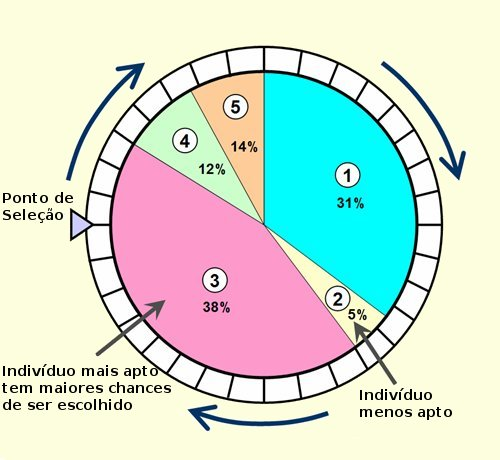
\includegraphics[scale=0.5]{images/roleta.jpg}
	\caption{Exemplo de seleção por roleta.}
	\label{fig:roleta}
\end{figure}


\pagestyle{plain}

\chapter{Implementações e Resultados Computacionais}\label{sec:resultados}

Nesta seção, apresentamos quatro algoritmos para a resolução do Problema da Mochila 0-1 e dois para o Problema da Mochila Compartimentada. O primeiro algoritmo, para ambas as versões, apresenta a resolução mais óbvia, os quais são implementados utilizando método ``força bruta'', ou seja, verifica todas as possíveis soluções e escolhe dentre elas, a melhor. Estes algoritmos encontram a solução exata, porém possuem complexidade de tempo exponencial.

O segundo e o terceiro algoritmos referem-se à resolução do Problema da Mochila 0-1 utilizando programação dinâmica e \textit{branch-and-bound}, respectivamente. Ambos os algoritmos também encontram a melhor solução, com desempenho muito melhor quando comparados ao algoritmo que utiliza a força bruta. No caso do \textit{branch-and-bound}, encontrar a solução ótima depende do cálculo do limitante. Se este não for justo, o tempo de execução pode ficar muito grande. Já com a programação dinâmica, o tempo de execução aumenta em função da quantidade de itens do conjunto e da capacidade máxima da mochila. Embora seja conhecido como um algoritmo ``pseudopolinomial'', por depender não só da quantidade de itens como também da capacidade da mochila, esse algoritmo executa rapidamente na prática. 

Os dois últimos referem-se a algoritmos genéticos para resolver tanto o Problema da Mochila 0-1 quanto o Problema da Mochila Compartimentada. Algoritmos genéticos não garantem que a melhor solução será encontrada, porém quanto maior o número de iterações ou gerações, a solução retornada pelo método tende ao valor ótimo.  Este tipo de algoritmo utiliza várias operações baseadas em probabilidade e operações aleatórias, que influenciam no resultado obtido. A maioria das operações simula os eventos que ocorrem no processo de evolução, 

Para podermos avaliar os algoritmos genéticos, denominaremos de {\it razão de aproximação} a divisão do valor da solução ótima pelo valor retornado pelo algoritmo genético. Já que os problemas em questão são de maximização, a razão de aproximação será um valor $\geq 1$. Quanto mais próximo de 1, mais próximo do valor ótimo será a resposta do algoritmo genético.


\section{Implementações da Mochila 0-1}

\subsection{Mochila 0-1 usando Força Bruta} \label{imp:force}
Um algoritmo que implementa a resolução de um problema através da força bruta é aquele que verifica todas as possíveis soluções e escolhe, dentre ela, a melhor. 

Para o Problema da Mochila 0-1, o algoritmo da força bruta compara todas as possibilidades de preenchimento da mochila que não ultrapassem o peso máximo estipulado. Durante este teste, o algoritmo guarda numa variável a maior utilidade obtida e ao final de todas as comparações, o resultado do algoritmo está armazenado nesta variável.

Não utiliza-se nenhuma estrutura de dados especial, apenas utiliza-se uma variável inteira para armazenar a maior utilidade encontrada até aquele momento da comparação.

\begin{algorithm}
\caption{Mochila\_Recursiva} %titulo do algoritmo
\label{alg1}
\scriptsize
\begin{algorithmic}[1]

  \REQUIRE Os vetores de benefícios $(p)$ e de peso $(w)$, o número de itens $(n)$ e o limite da mochila $(W)$.
	\ENSURE O benefício total.

  \IF{$n == 0$}
    \RETURN $0$
	\ENDIF

  \STATE $a = Mochila\_Recursiva(a, b, p, w, n-1, W)$
  \IF{$w[n] > W$}
    \RETURN $a$
  \ELSE
    \STATE $b = v[n] + Mochila\_Recursiva(a, b, p, w, n-1, W-w[n])$
    \RETURN $max(a, b)$
  \ENDIF

\end{algorithmic}
\end{algorithm}

\subsection{Mochila 0-1 usando Programação Dinâmica}
O algoritmo usando programação dinâmica fornece a solução exata para o problema em tempo pseudo-polinomial, a complexidade varia de acordo com o tamanho da mochila e com o número de objetos. A implementação deste método refere-se á codificação em linguagem C do algoritmo apresentado na seção~\ref{progdin}.


\subsection{Mochila 0-1 usando Branch and Bound}

O algoritmo de \textit{branch-and-bound} funciona como o força bruta, porém inclui mecanismos para evitar descer na árvore de recursão desnecessariamente. A implementação usada é uma codificação, para C, do algoritmo apresentado em ~\cite{MTG02}.

\begin{algorithm}
\caption{Mochila\_Branch\_and\_Bound} %titulo do algoritmo
\label{alg3}
\scriptsize
\begin{algorithmic}[1]

  \REQUIRE Os vetores de benefícios $(v)$ e de peso $(w)$, o número de itens $(n)$ e o limite da mochila $(W)$.
	\ENSURE O benefício total.

	\STATE $maxprof = 0$
  \STATE $v.l = v.v = v.w = 0$
  \STATE $v.bound = Bound(v, p, w, n, W)$
  \STATE $push(v)$

  \WHILE{$size != 0$}

    \STATE $pop()$
    \STATE $v.v = q[size].v$
    \STATE $v.w = q[size].w$
    \STATE $v.l = q[size].l$
    \STATE $v.bound = q[size].bound$

    \IF{$v.bound > maxprof$}
      \STATE $u.l = v.l + 1$
      \STATE $u.w = v.w + w[u.l]$
      \STATE $u.v = v.v + p[u.l]$

      \IF{$u.w \leq W \ \&\& \ u.v > maxprof$}
				\STATE $maxprof = u.v$
			\ENDIF

      \STATE $u.bound = Bound(u, p, w, n, W)$
      \IF{$u.bound > maxprof$}
				\STATE $push(u)$
			\ENDIF

      \STATE $u.w = v.w$
      \STATE $u.v = v.v$
      \STATE $u.bound = Bound(u, p, w, n, W)$
      \IF{$u.bound > maxprof$}
				\STATE $push(u)$
			\ENDIF
    \ENDIF
  \ENDWHILE
  \RETURN maxprof

\end{algorithmic}
\end{algorithm}

\begin{algorithm}
\caption{Bound} %titulo do algoritmo
\label{alg4}
\scriptsize
\begin{algorithmic}[1]
	\REQUIRE O nó $(v)$, os vetores de benefícios $(v)$ e de peso $(w)$, o número de itens $(n)$ e o limite da mochila $(W)$.
	\ENSURE A pontuação do nó.

	\IF{$u.w \geq W$}
    \RETURN $0$
  \ELSE
    \STATE $result = u.v$
    \STATE $i = u.l + 1$
    \STATE $total = u.w$

    \WHILE{$i \leq n \ \&\& \ (total + w[i] \leq W)$}
      \STATE $total += w[i]$
      \STATE $result += v[i]$
    \ENDWHILE

    \STATE $j = i$
    \IF{$j \leq n$}
			\STATE $result += (W - total) * v[j]/w[j]$
		\ENDIF

    \RETURN result
  \ENDIF

\end{algorithmic}
\end{algorithm}

\newpage

\subsection{Mochila 0-1 usando Algoritmo Genético} \label{cap4:gen}

Segundo ~\cite{Wei09}, algoritmos genéticos são uma subclasse dos algoritmos evolucionários, onde o espaço de procura é um vetor de binários ou outros tipos elementares.

A implementação deste algoritmo tem sua formulação em~\cite{KJBR08}, onde são definidas as duas funções-objetivo:

\begin{eqnarray}
	Maximizar & \displaystyle \sum_{j = 1}^{n}p_{j}x_{j} \\
	Minimizar & \displaystyle \sum_{j = 1}^{n}w_{j}x_{j}
\end{eqnarray}

Onde a variável de decisão $x_{i}$, $i = 1, ..., n$, descreve se o item pertence a solução, $x_{i} = 1$, ou não, $x_{i} = 0$. Isto é, o algoritmo tenta maximizar o benefício enquanto minimiza o peso da mochila. O algoritmo 6 também é descrito por ~\cite{KJBR08}, onde é feito o cálculo das aptidões dos indivíduos da população. Essas aptidões, uma para o peso e outra para o benefício, após serem calculadas são normalizados, entre 0 e 1, onde 0 indica o melhor e 1 indica o pior valor. Com essa formulação das funções objetivo, a otimização se torna uma minimização em ambos as funções.

\begin{algorithm}[htp]
\caption{Mochila\_Genético\_Estrutura\_Básica} %titulo do algoritmo
\label{alg5}
\scriptsize
\begin{algorithmic}[1]

  \FOR{$i = 0 \ at\acute{e} \ generation\_size$}
		\STATE Avalie
		\STATE Reproduza
	\ENDFOR

\end{algorithmic}
\end{algorithm}

\begin{algorithm}
\caption{Avalie} %titulo do algoritmo
\scriptsize
\label{alg6}
\begin{algorithmic}[1]

  \STATE $maxprofit = 0$

  \FOR{$i = 0 \ at\acute{e} \ population\_size$}
    \STATE $profitFitness[i] = 0$
    \STATE $weightFitness[i] = 0$

		\STATE $cur[i].profit += v[j]$ % Verificar como colocar isso depois 
		\STATE $cur[i].weight += w[j]$

    \IF{$weight[i] > W$}
      \STATE $weight[i] = -(weight[i] - W)$
		\ENDIF

    \IF{$maxprofit < profit[i]$}
      \STATE $maxprofit = profit[i]$
		\ENDIF
  \ENDFOR

  \FOR{$i = 0 \ at\acute{e} \ population\_size$}
    \STATE $profitFitness[i] = 1 - (profit[i] / maxprofit) / psize$
    \STATE $weightFitness[i] = (weight[i] / W) / psize$
  \ENDFOR

\end{algorithmic}
\end{algorithm}

\begin{algorithm}
\caption{Reproduza} %titulo do algoritmo
\label{alg7}
\scriptsize
\begin{algorithmic}[1]

  \FOR{$i = 0 \ at\acute{e} \ population\_size$}
		\IF{($rand() \ \% \ 101) \leq 75$}
			\STATE Troca $k$ cromossomos entre os indivíduos $i$ e $i + 1$
		\ENDIF
		\FOR{$j = 1 \ at\acute{e} \ cromossome\_size$}
			\IF{()$rand() \ \% \ 101) \leq 5$}
				\STATE Inverte o $j$-ésimo cromossomo do indvíduo
			\ENDIF
		\ENDFOR
	\ENDFOR

\end{algorithmic}
\end{algorithm}

\newpage

\subsection{Comparações relevantes}

As simulações computacionais foram feitas em um computador com processador AMD Sempron(tm) Processor 2800 e 1GB de memória. Foram feitas cinco mochilas de pesos 50, 100, 150, 500 e 1000, com 25 casos de teste para cada mochila. Os valores para o número de itens e para seus pesos e benefícios foram gerados aleatoriamente. Para o Problema da Mochila, o algoritmo genético implementado gera soluções próximas as ótimas, sempre menores que uma 2-aproximação. O método de força bruta executou até a mochila de peso 100, devido ao seu tempo de execução exponencial, os outros métodos executaram todas as mochilas. Para essas simulações, o algoritmo genético utiliza os seguintes parâmetros:

\begin{itemize}
	\item Número de gerações: 50.
	\item Tamanho da população: 30.
	\item Taxa de \textit{cross-over}: 75\%.
	\item Taxa de mutação: 5\%.
\end{itemize}

Na figura~\ref{fig:w50}, podemos ver que, para uma mochila de peso limite igual a 50, o algoritmo com melhor tempo é o algoritmo que utiliza programação dinâmica, seguido pelo algoritmo que utiliza \textit{branch-and-bound}. Também podemos ver que, para essa mochila, o algoritmo genético manteve tempo quase constante e melhor que o tempo do algoritmo que utiliza força bruta, chegando a empatar, no tempo, com o algoritmo que utiliza \textit{branch-and-bound}. As soluções geradas com o algoritmo genético em 60\% dos casos de teste foram as soluções ótimas.

\begin{figure}[htp]
	\centering
	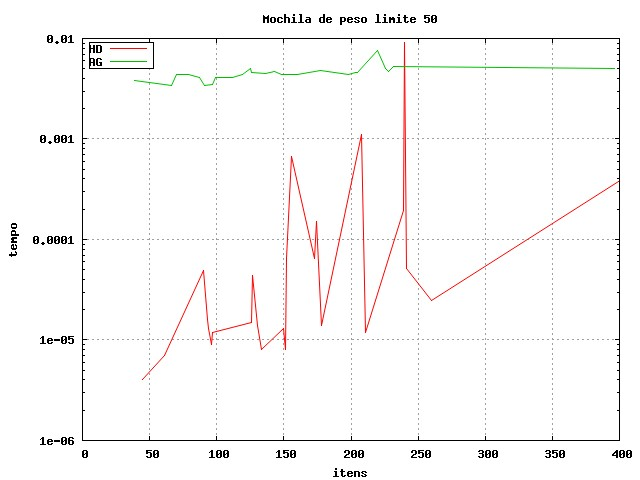
\includegraphics[scale=0.4]{images/w50.jpg}
	\caption{Gráfico comparativo dos tempos de execução dos quatro métodos: força bruta(FB), branch-and-bound(BB), programação dinâmica(PD) e algoritmos genéticos(AG), para mochilas com capacidade 50.}
	\label{fig:w50}
\end{figure}

Na figura~\ref{fig:w100}, podemos ver que o algoritmo genético obtêm tempo melhor que o algoritmo que utiliza \textit{branch-and-bound} a partir de 55 itens, mas que ainda se mantêm distante do tempo do algoritmo que utiliza programação dinâmica. Para esse tipo de mochila, o algoritmo genético gerou, em 24\% dos casos de teste, as soluções ótimas.

\begin{figure}[htp]
	\centering
	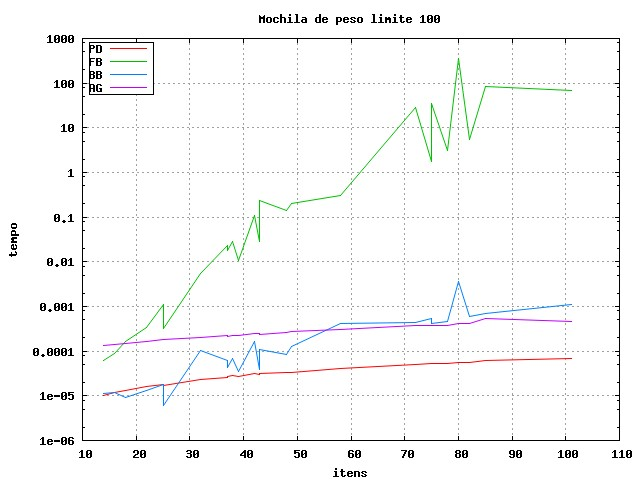
\includegraphics[scale=0.4]{images/w100.jpg}
	\caption{Gráfico comparativo dos tempos de execução dos quatro métodos: força bruta(FB), branch-and-bound(BB), programação dinâmica(PD) e algoritmos genéticos(AG), para mochilas com capacidade 100.}
	\label{fig:w100}
\end{figure}

Na figura~\ref{fig:w150}, em comparação com a figura~\ref{fig:w100}, podemos ver como o tempo do algoritmo genético começa a se aproximar do tempo do algoritmo que utiliza programação distribuida. O algoritmo genético gerou apenas uma solução ótima para esses casos de teste.

\begin{figure}[htp]
	\centering
	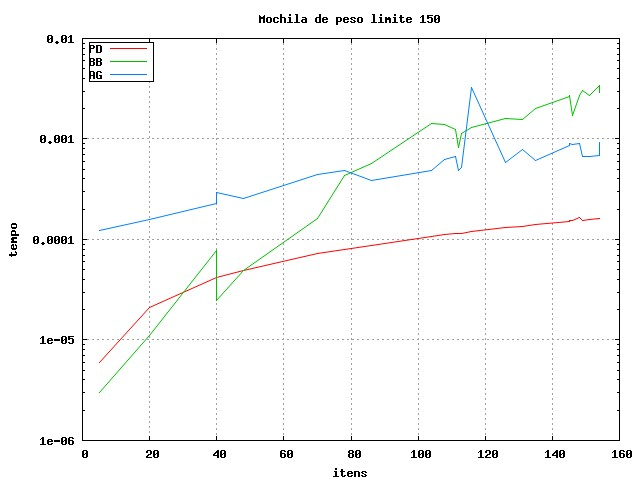
\includegraphics[scale=0.4]{images/w150.jpg}
	\caption{Gráfico comparativo dos tempos de execução dos três métodos mais rápidos: branch-and-bound(BB), programação dinâmica(PD) e algoritmos genéticos(AG), para mochilas com capacidade 150.}
	\label{fig:w150}
\end{figure}

Na figura~\ref{fig:w500}, podemos ver uma aproximação dos tempos de execução do algoritmo genético com o algoritmo que utiliza programação dinâmica. O algoritmo que utiliza \textit{branch-and-bound} é mais rápido para esse tipo de mochila quando o número de itens não ultrapassa 150. A partir desse ponto, o algoritmo se torna uma mais lento que os outros dois. Para esses casos de teste o algoritmo genético não gerou nenhuma solução ótima.

\begin{figure}[htp]
	\centering
	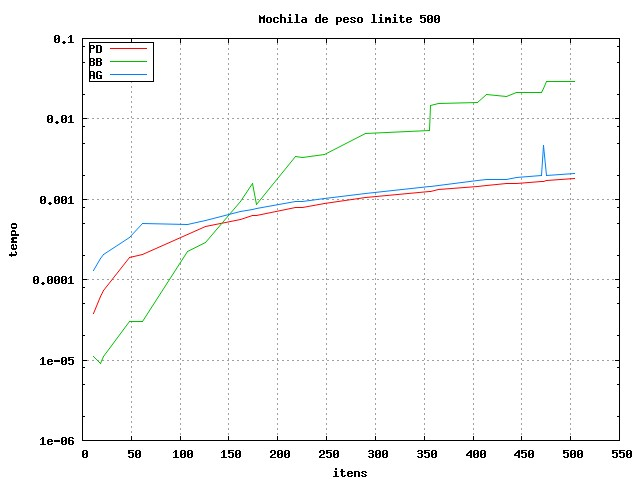
\includegraphics[scale=0.4]{images/w500.jpg}
	\caption{Gráfico comparativo dos tempos de execução dos três métodos mais rápidos: branch-and-bound(BB), programação dinâmica(PD) e algoritmos genéticos(AG), para mochilas com capacidade 500.}
	\label{fig:w500}
\end{figure}

Como podemos ver na figura~\ref{fig:w1000}, o algoritmo genético fica mais rápido que o algoritmo que utiliza programação dinâmica para quantidades grandes de itens e limites da mochila altos. o algoritmo que utiliza \textit{branch-and-bound} apresenta o mesmo comportamento que nas figuras anteriores, começa sendo rápido para uma quantidade pequena de itens e, a partir de um certo número de itens, tem o tempo maior que os outros dois algoritmos. Assim como nos casos de teste da mochila anterior, o algoritmo genético não encontrou nenhuma solução ótima.

\begin{figure}[htp]
	\centering
	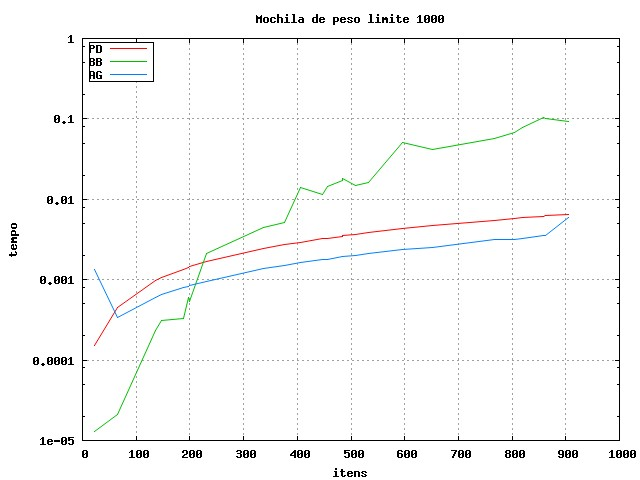
\includegraphics[scale=0.4]{images/w1000.jpg}
	\caption{Gráfico comparativo dos tempos de execução dos três métodos mais rápidos: branch-and-bound(BB), programação dinâmica(PD) e algoritmos genéticos(AG), para mochilas com capacidade 1000.}
	\label{fig:w1000}
\end{figure}

\newpage

\section{Mochila Compartimentada}
\subsection{Mochila Compartimentada usando Heurística da Decomposição}
A implementação deste algoritmo foi feita utilizando $K - 1$ chamadas ao algoritmo 1, que utiliza força bruta, uma para cada agrupamento de itens, para que fossem escolhidas os melhores compartimentos de cada agrupamento. Com esses compartimentos armazenados em um vetor, foi feita uma última chamada ao mesmo algoritmo, para que fossem escolhidos os compartimentos que entrariam na mochila.

\subsection{Mochila Compartimentada usando Algoritmo Genético}
Esse algoritmo genético é uma modificação do algoritmo da seção~\ref{cap4:gen}. Os pesos de cada compartimento são verificados e, se ultrapassarem o limite do compartimento, também sofrem penalidades. Com exeção dessa nova restrição, o algoritmo permanece o mesmo.


\begin{algorithm}
\caption{Avalie\_Compartimentada} %titulo do algoritmo
\scriptsize
\begin{algorithmic}[1]

  \STATE $maxprofit = 1$

  \FOR{$i = 0 \ at\acute{e} \ population\_size$}
    \STATE $profitFitness[i] = 0$
    \STATE $weightFitness[i] = 0$

    \WHILE{$!(stop) \&\& (j <= csize)$}

      \IF{$cur[i].cromo[j]$}

				\IF{$cur[i].type[itens[j].k] == 0$}
					\STATE $cur[i].type[itens[j].k] = 1$
					\STATE $cur[i].weight += S + itens[j].w$
					\STATE $cur[i].stype[itens[j].k] += S + itens[j].w$
					\STATE $cur[i].profit += (itens[j].p - c[itens[j].k])$
				\ELSE
					\STATE $cur[i].profit += itens[j].p$
					\STATE $cur[i].weight += itens[j].w$
					\STATE $cur[i].stype[itens[j].k] += itens[j].w$
				\ENDIF

				\IF{$cur[i].stype[itens[j].k] > L[itens[j].k]$}
					\STATE $cur[i].profit = 0$
					\STATE $cur[i].weight = 1$
					\STATE $stop = 0$
				\ENDIF
			\ENDIF
			\STATE $j++$
    \ENDWHILE

    \IF{$weight[i] > W$}
      \STATE $weight[i] = -(weight[i] - W)$
		\ENDIF

    \IF{$maxprofit < profit[i]$}
      \STATE $maxprofit = profit[i]$
		\ENDIF
  \ENDFOR

  \FOR{$i = 0 \ at\acute{e} population\_size$}
    \STATE $profitFitness[i] = 1 - (profit[i] / maxprofit) / psize$
    \STATE $weightFitness[i] = (weight[i] / W) / psize$
  \ENDFOR

\end{algorithmic}
\end{algorithm}


\subsection{Comparações relevantes}
As simulações computacionais foram feitas em um computador com processador AMD Sempron(tm) Processor 2800 e 1GB de memória. Foram feitas duas mochilas de pesos 50 e 100, com 25 casos de teste para cada mochila. Os valores para o número de itens e para seus pesos e benefícios foram gerados aleatoriamente.

\begin{itemize}
	\item Número de gerações: 50.
	\item Tamanho da população: 30.
	\item Taxa de \textit{cross-over}: 60\%.
	\item Taxa de mutação: 5\%.
\end{itemize}

Na figura~\ref{fig:com_w50}, vemos que o algoritmo genético não é tão eficiente para mochilas pequenas, uma vez que para verificar se uma configuração da mochila é válida o tempo gasto é grande. O algoritmo genético para ela encontrou a solução ótima em apenas um caso de teste, com razão de aproximação próxima a 1 em 44\% dos casos e, nos demais, com razão de aproximação próxima a 2. 

\begin{figure}[htp]
	\centering
	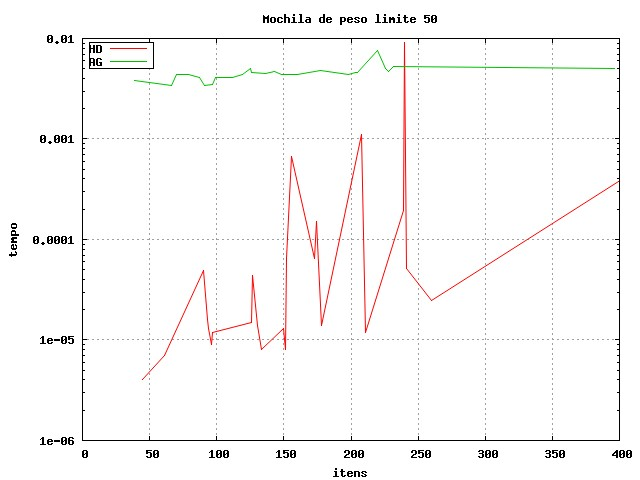
\includegraphics[scale=0.4]{images/com_w50.jpg}
	\caption{Gráfico comparativo dos tempos de execução dos dois métodos: heurística da decomposição(HD) e algoritmos genéticos(AG), para mochilas com capacidade 50.}
	\label{fig:com_w50}
\end{figure}

Com o aumento no número de itens e no limite da mochila, o algoritmo genético permanece com o mesmo tempo dos teste com a mochila de peso limite igual a 50, como podemos ver na figura~\ref{fig:com_w100}. Ao mesmo tempo, podemos ver o aumento no tempo de execução do algoritmo que utiliza a heurística da decomposição. Assim como na mochila anterior, o algoritmo genético encontrou a solução ótima em apenas um caso e, em 52\% dos casos, encontrou uma solução com razão de aproximação próxima a 2.

\begin{figure}[htp]
	\centering
	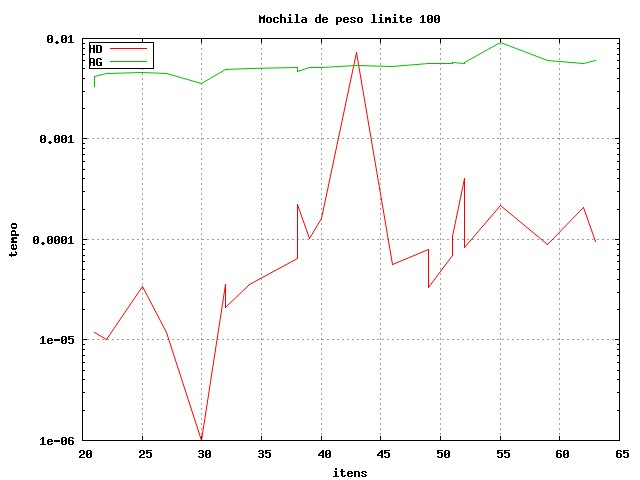
\includegraphics[scale=0.4]{images/com_w100.jpg}
	\caption{Gráfico comparativo dos tempos de execução dos dois métodos: heurística da decomposição(HD) e algoritmos genéticos(AG), para mochilas com capacidade 100.}
	\label{fig:com_w100}
\end{figure}

%Na figura~\ref{fig:com_w150}, podemos ver que, para alguns casos, o tempo de execução do algoritmo genético é melhor do que o tempo do algoritmo que utiliza a heurística da decomposição. Porém, o algoritmo genético não gerou nenhuma solução ótima para esse tipo de mochila.

%\begin{figure}[htp]
%	\centering
%	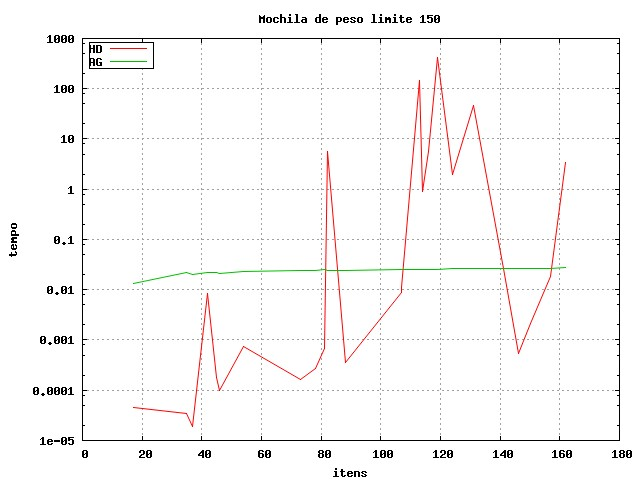
\includegraphics[scale=0.4]{images/com_w150.jpg}
%	\caption{Gráfico comparativo dos tempos de execução dos dois métodos: heurística da decomposição(HD) e algoritmos genéticos(AG), para mochilas com capacidade 150.}
%	\label{fig:com_w150}
%\end{figure}

\pagestyle{plain}

\chapter{Considerações Finais} \label{sec:conclusao}

Este trabalho abordou o Problema da Mochila clássico e uma variação do mesmo, denominada Problema da Mochila Compartimentada. Ambos são problemas de otimização combinatória pertencentes à classe NP-difícil e possuem importantes aplicações práticas.

Após uma revisão bibliográfica sobre as principais estratégias para resolução de Problemas da Mochila, vários experimentações foram realizadas a fim de avaliar estas técnicas e melhorar o tempo de resposta dos métodos tradicionais. Visto que estes problemas aparecem como sub-problemas de vários outros, justifica-se a tentativa de encontrar heurísticas e algoritmos aproximados com boas razões de aproximação para resolvê-los. A proposta de implementação de um algoritmo genético para esses problemas contribui de duas formas: bom desempenho quando comparado com às implementações tradicionais e boas aproximações com relação aos valores retornados como saída.

Para o Problema da Mochila 0-1, o algoritmo genético apresentou bons resultados, retornando a solução ótima na maior parte dos casos e com bom desempenho. Utilizamos a razão de aproximação para avaliar quão boa foi a resposta dos nossos métodos. No caso do Problema da Mochila 0-1, a razão de aproximação obtida foi igual a 1,13. Com relação ao Problema da Mochila Compartimentada, o algoritmo genético apresentou bom desempenho, porém não há como avaliar com precisão quão próxima da solução ótima está a resposta do algoritmo, dado que o resultado retornado foi comparadado com a resposta do programa utilizando a heurística da decomposição, que não garante a solução ótima em todos os casos. Ainda assim, o algoritmo genético  retornou, em média, soluções com uma razão de aproximação próxima a 2.

Embora os algoritmos genéticos tenham apresentado boas razões de aproximação, não podemos dizer que sejam algoritmos aproximativos, pois os resultados apresentados são empíricos e não poderemos garantí-los sempre. 

Citamos como futuro trabalho a melhoria dos parâmetros do algoritmo genético para o Problema da Mochila Compartimentada, para que venha a convergir mais rapidamente à solução ótima. Também seria interessante estender o algoritmo genético para que retornasse soluções sem considerar as simplificações na modelagem matemática que aqui foram adotadas.

% \section{Contribuições do Trabalho}
% \section{Limitações do Trabalho}
% \section{Trabalhos futuros} \label{sec:trabafuturos}

\nocite{*}
%\bibliographystyle{unsrt}
%\bibliographystyle{plain}
\bibliographystyle{alpha}
%\bibliographystyle{acm}
%\bibliographystyle{abbrv}
%\bibliographystyle{apalike}
\bibliography{referencia}

%\input{apendice.tex}

\end{document}
